\chapter{Math test}

\section{Des propriétés}

\be\bmc{2}
\item Mais quoi ?
\item $\dfrac{3}{2}+\dfrac{13}{3}=\dfrac{35}{6}$
\emc\ee

\bi
\item Mais quoi ?
\item $\dfrac{3}{2}+\dfrac{13}{3}=\dfrac{35}{6}$
\ei

\section{Des propriétés}

\definition

Pour tout $a$ et $b\in\R$, on a : $$a^2+b^2 = c^2$$.

Le triangle $ABC$ est donc rectangle en $A$

\begin{marginfigure}
	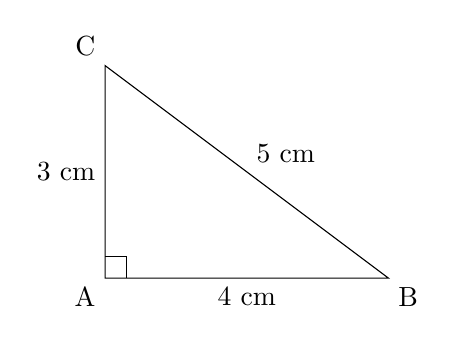
\begin{tikzpicture}[scale=0.9]
		\coordinate (A) at (0,0);
		\coordinate (B) at (4,0);
		\coordinate (C) at (0,3);
		\draw (A) -- (B) -- (C) -- cycle;
		\draw (0,0.3) -- (0.3,0.3) -- (0.3,0);
		\node[below left] at (A) {A};
		\node[below right] at (B) {B};
		\node[above left] at (C) {C};
		\node[below] at (2,0) {4 cm};
		\node[left] at (0,1.5) {3 cm};
		\node[above right] at (2,1.5) {5 cm};
	\end{tikzpicture}
	\caption{Un triangle rectangle}
\end{marginfigure}

\prop

plop

\ex \lipsum[2]

\rem Il faut faire attention aux nains\sidenote{Surtout celui-là\cimg{0.5\linewidth}{img/nain.png}}.

\methode

Pour additionner deux fractions, il faut les mettre sous même dénominateur.

\be\bmc{2}
\item $A=\dfrac{3}{2}+\dfrac{13}{3}$
\item $B=\dfrac{5}{7}-\dfrac{1}{5}$
\emc\ee
\ber\bmc{2}
\item $C=3-\dfrac{3}{10}$
\item $D=\dfrac{3}{2}+1$
\emc\ee

\correction\sidenote{\cimg{\linewidth}{img/plop}}

\be\bmc{2}
\item ~\\
$\def\arraystretch{2}
	\begin{array}{rcl}
		A & = & \dfrac{3}{2}+\dfrac{13}{3}                       \\
		  & = & \dfrac{9}{6}+\dfrac{26}{6} \quad = \dfrac{35}{6}
	\end{array}$
\item ~\\
$\def\arraystretch{2}
	\begin{array}{rcl}
		B & = & \dfrac{5}{7}-\dfrac{1}{5}                             \\
		  & = & \dfrac{25}{35}+\dfrac{7}{35}  \quad =  \dfrac{18}{35}
	\end{array}$
\emc\ee

% \begin{marginfigure}\cimg{\linewidth}{img/16.png}\end{marginfigure}

\ber\bmc{2}
\item ~\\
$\def\arraystretch{2}
	\begin{array}{rcl}
		C & = & 3-\dfrac{3}{10}                                     \\
		  & = & \dfrac{30}{10}+\dfrac{3}{10} \quad = \dfrac{33}{10}
	\end{array}$
\item ~\\
$\def\arraystretch{2}
	\begin{array}{rcl}
		D & = & \dfrac{3}{2}+1                              \\
		  & = & \dfrac{3}{2}+\dfrac{2}{2} \quad = \dfrac{5}{2}
	\end{array}$
\emc\ee

Mais c'est trop!!!!\citation{Mr andrews}


